%%%%%%%%%%%%%%%%%%%%%%%%%%%%%%%%%%%%%%%%%
% Jacobs Landscape Poster
% LaTeX Template
% Version 1.1 (14/06/14)
%
% Created by:
% Computational Physics and Biophysics Group, Jacobs University
% https://teamwork.jacobs-university.de:8443/confluence/display/CoPandBiG/LaTeX+Poster
% 
% Further modified by:
% Nathaniel Johnston (nathaniel@njohnston.ca)
%
% This template has been downloaded from:
% http://www.LaTeXTemplates.com
%
% License:
% CC BY-NC-SA 3.0 (http://creativecommons.org/licenses/by-nc-sa/3.0/)
%
%%%%%%%%%%%%%%%%%%%%%%%%%%%%%%%%%%%%%%%%%

%----------------------------------------------------------------------------------------
%	PACKAGES AND OTHER DOCUMENT CONFIGURATIONS
%----------------------------------------------------------------------------------------

\documentclass[final]{beamer}

\usepackage{pifont} % for dings

\usepackage[scale=1.24]{beamerposter} % Use the beamerposter package for laying out the poster

\usetheme{confposter} % Use the confposter theme supplied with this template

\setbeamercolor{block title}{fg=ngreen,bg=white} % Colors of the block titles
\setbeamercolor{block body}{fg=black,bg=white} % Colors of the body of blocks
\setbeamercolor{block alerted title}{fg=white,bg=dblue!70} % Colors of the highlighted block titles
\setbeamercolor{block alerted body}{fg=black,bg=dblue!10} % Colors of the body of highlighted blocks
% Many more colors are available for use in beamerthemeconfposter.sty

%-----------------------------------------------------------
% Define the column widths and overall poster size
% To set effective sepwid, onecolwid and twocolwid values, first choose how many columns you want and how much separation you want between columns
% In this template, the separation width chosen is 0.024 of the paper width and a 4-column layout
% onecolwid should therefore be (1-(# of columns+1)*sepwid)/# of columns e.g. (1-(4+1)*0.024)/4 = 0.22
% Set twocolwid to be (2*onecolwid)+sepwid = 0.464
% Set threecolwid to be (3*onecolwid)+2*sepwid = 0.708

\newlength{\sepwid}
\newlength{\onecolwid}
\newlength{\twocolwid}
\newlength{\threecolwid}
\setlength{\paperwidth}{48in} % A0 width: 46.8in
\setlength{\paperheight}{36in} % A0 height: 33.1in
\setlength{\sepwid}{0.024\paperwidth} % Separation width (white space) between columns
\setlength{\onecolwid}{0.22\paperwidth} % Width of one column
\setlength{\twocolwid}{0.464\paperwidth} % Width of two columns
\setlength{\threecolwid}{0.708\paperwidth} % Width of three columns
\setlength{\topmargin}{-0.5in} % Reduce the top margin size
%-----------------------------------------------------------

\usepackage{graphicx}  % Required for including images

\usepackage{booktabs} % Top and bottom rules for tables

%----------------------------------------------------------------------------------------
%	TITLE SECTION 
%----------------------------------------------------------------------------------------

\title{Survival Analysis of Questions Posted on the iFixit Answers Forum} % Poster title

\author{Lisa Oshita\footnote{Frost Research Fellow, recipient of the Frost Undergraduate Student Research Award}, Anthony Pileggi, Shannon Pileggi} % Author(s)

\institute{Department of Statistics, California Polytechnic State University} % Institution(s)

%----------------------------------------------------------------------------------------

\begin{document}

\addtobeamertemplate{block end}{}{\vspace*{2ex}} % White space under blocks
\addtobeamertemplate{block alerted end}{}{\vspace*{2ex}} % White space under highlighted (alert) blocks

\setlength{\belowcaptionskip}{2ex} % White space under figures
\setlength\belowdisplayshortskip{2ex} % White space under equations

\begin{frame}[t] % The whole poster is enclosed in one beamer frame

\begin{columns}[t] % The whole poster consists of three major columns, the second of which is split into two columns twice - the [t] option aligns each column's content to the top

\begin{column}{\sepwid}\end{column} % Empty spacer column

\begin{column}{\onecolwid} % The first column

%----------------------------------------------------------------------------------------
%	OBJECTIVES
%----------------------------------------------------------------------------------------

\begin{alertblock}{Overview}

\textcolor{dblue!70}{\ding{228}} iFixit's online question and answer forum, \textit{Answers}, features over 120,000 user-asked questions related specifically to device repair. Analysis of question response times can reveal factors that affect how quickly questions receive answers, which can lead to suggestions for how users can ask better questions to minimize response times and for how forum design can be improved. 

\textcolor{dblue!70}{\ding{228}} \underline{Objective} Develop a Cox proportional hazards model to predict the survival probability, defined as the probability that a question remains unanswered beyond a certain time \textit{t}, of questions on the forum, with the goal of identifying variables signficantly associated with response time.

\end{alertblock}

%----------------------------------------------------------------------------------------
%	INTRODUCTION
%----------------------------------------------------------------------------------------

\begin{block}{Materials}

The data analyzed contained 8,025 questions posted from April 8, 2017 to July 7, 2017 (date of data download). Variables in the data included: device name, device category, question title, text, tags, new user status, date and time the question was posted, and date and time the first answer was received. Fourteen variables, capturing textual and user information of each question, were derived from the data.


% \textcolor{dblue!70}{\ding{228}} Device category the question pertains to
% 
% \textcolor{dblue!70}{\ding{228}} If the question was posted on a weekend or on a weekday
% 
% \textcolor{dblue!70}{\ding{228}} If the question's text contains end punctuation marks (. ? !)
% 
% \textcolor{dblue!70}{\ding{228}} If the question's text is in all lower case
% 
% \textcolor{dblue!70}{\ding{228}} If the question's title contains at least one word considered to be ``frequently-used'' among answered questions
% 
% \textcolor{dblue!70}{\ding{228}} If the question's title contains at least one word considered to be ``frequently-used'' among unanswered question
% 
% \textcolor{dblue!70}{\ding{228}} If the question's title ends in a question mark
% 
% \textcolor{dblue!70}{\ding{228}} If the user edited or added information to the question's text after posting it
% 
% \textcolor{dblue!70}{\ding{228}} If the suer made an effort to solve the problem prior to asking the question
% 
% \textcolor{dblue!70}{\ding{228}} Average tag length
% 
% \textcolor{dblue!70}{\ding{228}} Average tag frequency
% 
% \textcolor{dblue!70}{\ding{228}} Text length
% 
% \textcolor{dblue!70}{\ding{228}} Title length
% 
% \textcolor{dblue!70}{\ding{228}} Number of line breaks to text length ratio



\end{block}

%------------------------------------------------

\begin{figure}
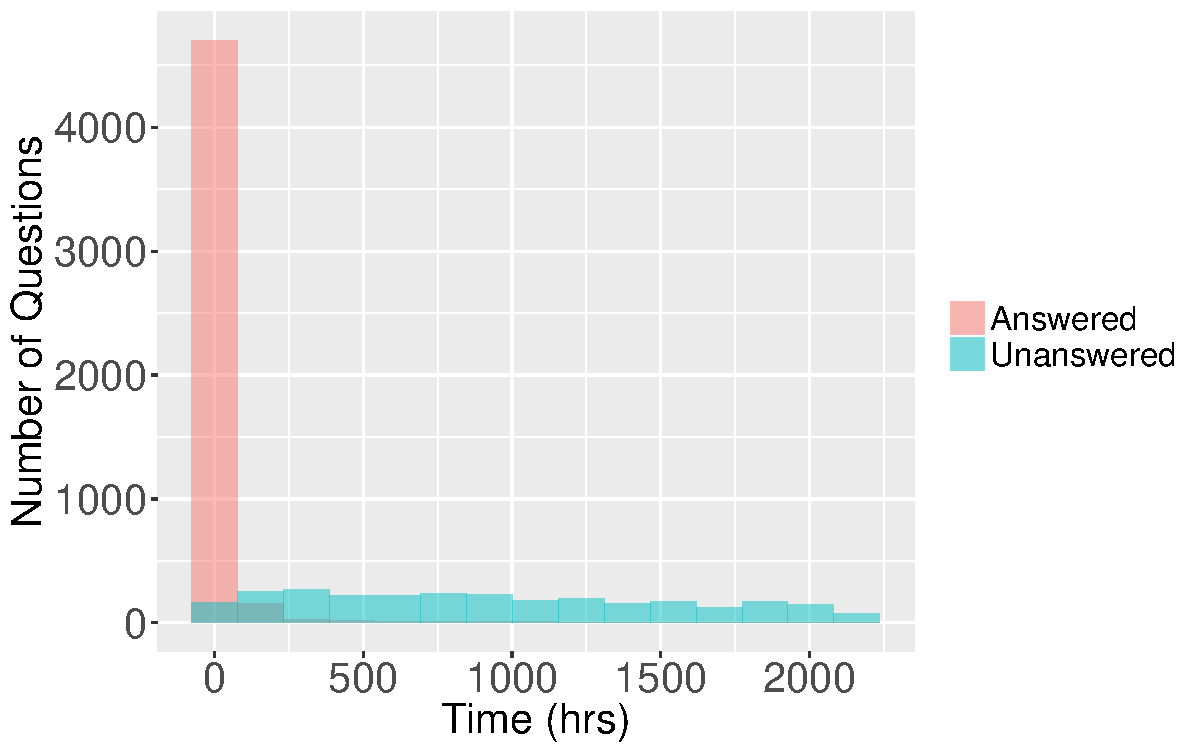
\includegraphics[width=1\linewidth]{FIG1.pdf}
\caption{Distribution of response times}
\label{fig1}
\end{figure}

%----------------------------------------------------------------------------------------

\end{column} % End of the first column

\begin{column}{\sepwid}\end{column} % Empty spacer column

\begin{column}{\twocolwid} % Begin a column which is two columns wide (column 2)

\begin{columns}[t,totalwidth=\twocolwid] % Split up the two columns wide column

\begin{column}{\onecolwid}\vspace{-.6in} % The first column within column 2 (column 2.1)

%----------------------------------------------------------------------------------------
%	METHODS
%----------------------------------------------------------------------------------------
\begin{block}{Model Building}

\textcolor{dblue!70}{\ding{228}} Univariate analysis was used to identify which variables, as well as the optimal form of continuous variables (if transformations and splines should be used), to include in the final Cox model for five fold cross-validation. 

\textcolor{dblue!70}{\ding{228}} In each iteration of cross-validation, the model was built on the training set and used to generate predicted hazard ratios on the corresponding test set. To assess performance, predicted hazard ratios were entered into separate Cox models as the single quantitative predictor with response times as the survival time. The resulting Nagelkerke's $R^2$ statistic, concordance statistic, Somers' \textit{Dxy}, partial likelihood ratio and p-value, were averaged over each iteration and assessed as indicators of the model's performance.  

\textcolor{dblue!70}{\ding{228}} The final model was fit to the full data and the proportional hazards assumption was assessed. 
\end{block}


\begin{block}{Results}

Of 7,760 questions in English, 4,951 (63.8\%) received an answer by the download date. The shortest response time was 0.5 hours. The longest was 2,159 hours (90 days). Figure 1 shows the distribution of response times for all questions analyzed. 

Univariate analysis determined that all categorical predictors were signficantly associated with response time. The following transformations were made to continous variables: 

\textcolor{dblue!70}{\ding{228}} $\sqrt{\textnormal{average tag frequency}}$

\textcolor{dblue!70}{\ding{228}} $\log\left({\textnormal{average tag length} + 1}\right)$, spline of 4 knots

\textcolor{dblue!70}{\ding{228}} $\log\left({\textnormal{device length} + 1}\right)$, spline of 5 knots

\textcolor{dblue!70}{\ding{228}} $\sqrt{\textnormal{line breaks / text length}}$, spline of 3 knots

\textcolor{dblue!70}{\ding{228}} $\log\left({\textnormal{text length}}\right)$, spline of 5 knots

Average performance metrics for test sets, training sets, as well as the full model are in Table \ref{table:1}. Partial likelihood ratios and p-values indicate that the model as a whole is significantly associated with response time. However, $R^2$ statistics and discrimination indexes are considerably low.

\end{block}


%----------------------------------------------------------------------------------------

\end{column} % End of column 2.1

\begin{column}{\onecolwid}\vspace{-.6in} % The second column within column 2 (column 2.2)

%----------------------------------------------------------------------------------------
%	Results
%----------------------------------------------------------------------------------------



% \begin{figure}
% 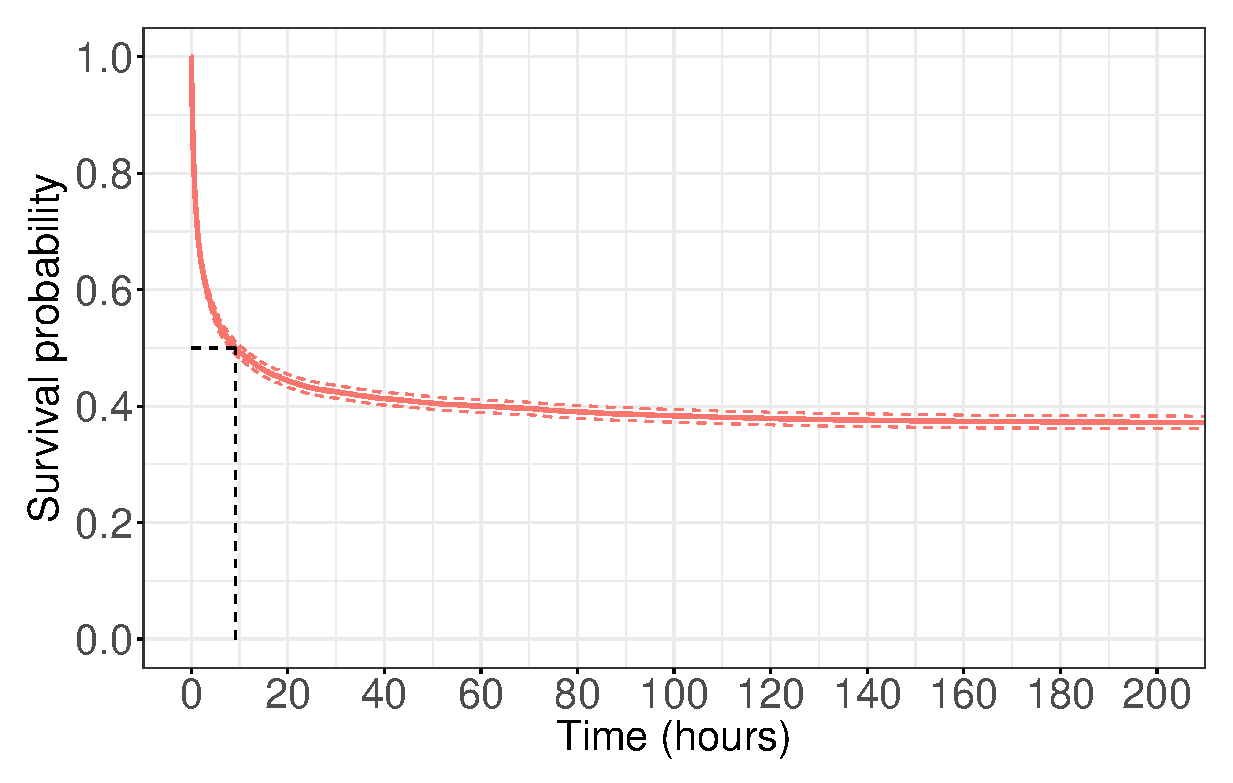
\includegraphics[width=0.99\linewidth]{FIG2.eps}
% \caption{Kaplan-Meier estimated survival probability curve. Median survival time indicated by the dotted line. }
% \end{figure}

\begin{block}

Results for training, test, and the full data did not change significantly, indicating that the model was not over fit. 

\end{block}


\begin{table}[!htbp]
\centering
\begin{tabular}{|r|r|r|r|r|r|r|r|}
  \hline
 & \textbf{HR} & \textbf{LR} & \textbf{p-value} & \textbf{$R^2$} & \textbf{\textit{Dxy}} & \textbf{C} \\ 
  \hline
  \textbf{Training} & 2.03 & 937.39  & \textless0.0001 & 0.14 & 0.27 & 0.63 \\ 
  \textbf{Test}     & 1.99 & 220.83  & \textless0.0001 & 0.14 & 0.26 & 0.63 \\
  \textbf{Full}     & 2.03 & 1165.03 & \textless0.0001 & 0.14 & 0.28 & 0.63 \\ 
   \hline
\end{tabular}
\caption{Performance metrics. (HR: Hazard Ratio, LR: Partial Likelihood Ratio, C: Concordance)} 
\label{table:1}
\end{table}

\begin{block}

Table 2 displays the coefficients for predictors in the final model fit to the full data. As a whole, the final model was significant with a partial likelihood ratio of 1265.29 (p-value \textless0.0001). Its $R^2$ statistic was 0.15, and Somers' \textit{Dxy} was 0.27. 

Assessing the proportional hazards assumption indicated that several levels of the device categorization variable, specifically Apple Product, Camera, Game Console, and Other, violated the assumption. 

The following are interpretations of select hazard coefficients in Table 2. Hazard is approximately equivalent to the conditional probability that a question will receive an answer within the next moment in time, given that it has not already received an answer. 

\textcolor{dblue!70}{\ding{228}} The estimated hazard of receiving an answer is 154\% higher (95\% CI (132\%, 179\%)) for questions pertaining to Apple products than the hazard for questions about Android and Other phones, controlling for all other predictors.

\textcolor{dblue!70}{\ding{228}} The estimated hazard of receiving an answer is 25\% lower (95\% CI (19\%, 29\%)) for questions with titles that contain at least one word considered to be frequently-used among unanswered questions, than the hazard for questions with titles that do not, controlling for all other predictors. 


\end{block}








%----------------------------------------------------------------------------------------

\end{column} % End of column 2.2

\end{columns} % End of the split of column 2 - any content after this will now take up 2 columns width

%----------------------------------------------------------------------------------------
%	IMPORTANT RESULT
%----------------------------------------------------------------------------------------

% \begin{alertblock}{Important Result}
% 
% Lorem ipsum dolor \textbf{sit amet}, consectetur adipiscing elit. Sed commodo molestie porta. Sed ultrices scelerisque sapien ac commodo. Donec ut volutpat elit.
% 
% \end{alertblock} 

%----------------------------------------------------------------------------------------

\begin{columns}[t,totalwidth=\twocolwid] % Split up the two columns wide column again

\begin{column}{\onecolwid} % The first column within column 2 (column 2.1)
%----------------------------------------------------------------------------------------

\end{column} % End of column 2.1

\begin{column}{\onecolwid} % The second column within column 2 (column 2.2)

%----------------------------------------------------------------------------------------
%	RESULTS
%----------------------------------------------------------------------------------------

% \begin{block}{Results}
% 
% 
% 
% Nunc tempus venenatis facilisis. Curabitur suscipit consequat eros non porttitor. Sed a massa dolor, id ornare enim:
% 
% \begin{table}
% \vspace{2ex}
% \begin{tabular}{l l l}
% \toprule
% \textbf{Treatments} & \textbf{Response 1} & \textbf{Response 2}\\
% \midrule
% Treatment 1 & 0.0003262 & 0.562 \\
% Treatment 2 & 0.0015681 & 0.910 \\
% Treatment 3 & 0.0009271 & 0.296 \\
% \bottomrule
% \end{tabular}
% \caption{Table caption}
% \end{table}
% 
% \end{block}

%----------------------------------------------------------------------------------------

\end{column} % End of column 2.2

\end{columns} % End of the split of column 2

\end{column} % End of the second column

\begin{column}{\sepwid}\end{column} % Empty spacer column

\begin{column}{\onecolwid} % The third column

%----------------------------------------------------------------------------------------
%	CONCLUSION
%----------------------------------------------------------------------------------------

\begin{block}{Discussion}

The model's weak predictive accuracy, which may be explained by limitations in the data, lead to suggestions for changes in CQA design. Many users incorrectly specified the device names and tags. It is likely that these inconsistencies contributed to the final model's low predictive power. As findings indicate that questions with correctly defined tags and device names may lead to quicker response times, the CQA can provide a stricter framework for asking questions by restricting the tags or devices that users can include to a drop-down list. The CQA can also include more tips to guide users asking questions. Implementing a more structured framework for asking questions can help users create understandable and clear questions and in turn decrease response time, as well as create a set of consistent questions for improved analysis. 

\end{block}


\begin{block}{Conclusion}

Predictors found to be significant in the final Cox regression model included: device category, if the question was posted on a weekend or a weekday, whether or not the question's title contained at least one word considered frequently-used among unanswered questions, and whether or not the question's title ends in a question mark. While overall the model was significant, its predictive performance was considerably low. 


\end{block}

%----------------------------------------------------------------------------------------
%	ADDITIONAL INFORMATION
%----------------------------------------------------------------------------------------

% \begin{block}{Additional Information}
% 
% Maecenas ultricies feugiat velit non mattis. Fusce tempus arcu id ligula varius dictum. 
% \begin{itemize}
% \item Curabitur pellentesque dignissim
% \item Eu facilisis est tempus quis
% \item Duis porta consequat lorem
% \end{itemize}
% 
% \end{block}

%----------------------------------------------------------------------------------------
%	REFERENCES
%----------------------------------------------------------------------------------------

% \begin{block}{References}
% 
% \nocite{*} % Insert publications even if they are not cited in the poster
% \small{\bibliographystyle{unsrt}
% \bibliography{sample}\vspace{0.75in}}
% 
% \end{block}

%----------------------------------------------------------------------------------------
%	ACKNOWLEDGEMENTS
%----------------------------------------------------------------------------------------

\setbeamercolor{block title}{fg=red,bg=white} % Change the block title color

\begin{block}{Acknowledgements}

\small{\rmfamily{This research was supported by the Bill and Linda Frost fund of the California Polytechnic State University of San Luis Obispo. We also thank iFixit for providing access to the CQA data.}} \\

\end{block}


%----------------------------------------------------------------------------------------
%	CONTACT INFORMATION
%----------------------------------------------------------------------------------------

% \setbeamercolor{block alerted title}{fg=black,bg=norange} % Change the alert block title colors
% \setbeamercolor{block alerted body}{fg=black,bg=white} % Change the alert block body colors
% 
% \begin{alertblock}{Contact Information}
% 
% \begin{itemize}
% \item Web: \href{http://www.university.edu/smithlab}{http://www.university.edu/smithlab}
% \item Email: \href{mailto:john@smith.com}{john@smith.com}
% \item Phone: +1 (000) 111 1111
% \end{itemize}
% 
% \end{alertblock}
% 
% \begin{center}
% \begin{tabular}{ccc}
% \includegraphics[width=0.4\linewidth]{logo.png} & \hfill & \includegraphics[width=0.4\linewidth]{logo.png}
% \end{tabular}
% \end{center}

%----------------------------------------------------------------------------------------

\end{column} % End of the third column

\end{columns} % End of all the columns in the poster

\end{frame} % End of the enclosing frame

\end{document}
